\subsection{Use cases}
	\lstinputlisting{usecases/cases.txt}
\subsection{Use case diagram}
	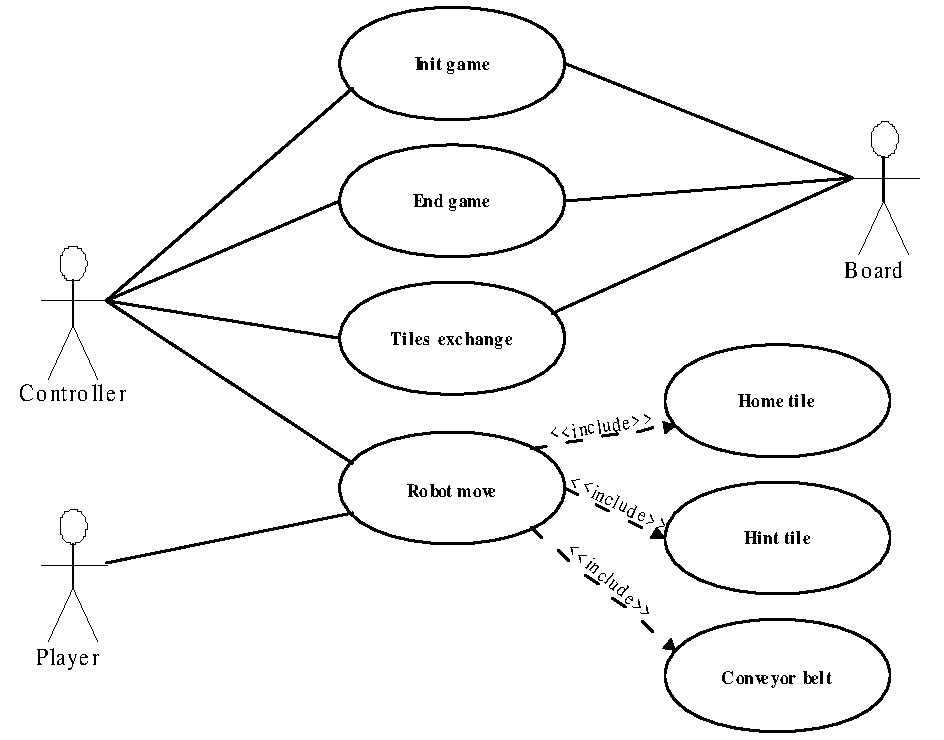
\includegraphics[width=\linewidth]{usecases/diagram.pdf}	

\subsection{High Level Message Sequence Chart}
	The following graph represents our high level message sequence chart and shows how a normal program flow is modeled by MSCs. The graph consists of two parts that run concurrently, the viewer part and the main game part. The viewer part will make sure the viewer updates regularly. The main game part follows the flow of a normal game. 
	
	\digraph[scale=0.4]{HMSC}{
begin2 [label="",shape="invtriangle"];
end2 [label="",shape="triangle"];
initview [label="Initialize viewer",shape="Mrecord"];
updateview [label="Update viewer",shape="Mrecord"];
begin2->initview;
initview->updateview;
updateview->updateview;
updateview->end2;
begin [label="",shape="invtriangle"];
end [label="",shape="triangle"];
p1 [label="",shape="point"];
p2 [label="",shape="point"];
p22 [label="",shape="point"];
p3 [label="",shape="point"];
p4 [label="",shape="point"];
p5 [label="",shape="point"];
p55 [label="",shape="point"];
p6 [label="",shape="point"];
p66 [label="",shape="point"];
p7 [label="",shape="point"];
p77 [label="",shape="point"];
p8 [label="",shape="point"];
init [label="Initialize",shape="Mrecord"];
mvreq [label="Robot move request",shape="Mrecord"];
mvrej [label="Reject move",shape="Mrecord"];
retnt [label="Return Normal tile",shape="Mrecord"];
retht [label="Return Hint tile",shape="Mrecord"];
retct [label="Return Conveyor tile",shape="Mrecord"];
retmt [label="Return Home tile",shape="Mrecord"];
ordex [label="Ordinary exchange",shape="Mrecord"];
spcex [label="Special exchange",shape="Mrecord"];
endgame [label="End game",shape="Mrecord"];
notrob1 [label="Notify robots",shape="Mrecord"];
notrob2 [label="Notify robots",shape="Mrecord"];
begin->p1;
p1->init;
init->p2;
p2->mvreq;
mvreq->p3;
p3->mvrej;
mvrej->p2;
p3->p4;
p4->retnt;
p4->retht;
p4->retct;
p4->retmt;
retnt->p5;
retht->p5;
retct->p5;
p5->p55;
p55->p66;
p66->p6;
p55->notrob1;
notrob1->p66;
p6->ordex;
p6->spcex;
ordex->p7;
spcex->p7;
p7->p77;
p77->p22;
p22->p2 [tailport=e];
p77->notrob2;
notrob2->p22;
retmt->endgame;
endgame->p8;
p8->p1;
p8->end;
}

	
\subsection{Message Sequence Charts}
	This section contains the message sequence charts for our use cases. Below every MSC is the location of the MSC in the High Level Message Sequence Chart.

	The world entity is not a real part of our MSCs, but rather a link to the outside world. When an internal action ends in '()' it's a function call to a private function of the entity. Otherwise, it's an action within the called function.

	Note: the symbol $\vdots$ denotes the start and end of a co-region.

	\subsubsection{Initialize viewer}
	The viewer is initialized by the world. Analogous to the HMSC, this happens concurrently to the Initialize MSC.
	
	\begin{msc}
msc
{

w [label="World"],
b [label="Board"],
c [label="Controller"],
v [label="Viewer"];

v box v [label=""],
b box b [label=""],
c box c [label=""],
w box w [label=""];

|||;

w => v [label="initialize(controller)"];
v rbox v [label="initialize"];
v => c [label="addViewer(viewer)"];
c >> v [label="self"];

... [label="board waits a predefined time"];

b rbox b [label="make snapshot"];
b -> c [label="notifyViewer(snapshot)"];
c -> v [label="notifyStateChange(snapshot)"];
v rbox v [label="updateView()"];

|||;

v box v [label="", textbgcolor="black"],
b box b [label="", textbgcolor="black"],
c box c [label="", textbgcolor="black"],
w box w [label="", textbgcolor="black"];

}
\end{msc}
\digraph[scale=0.5]{HMSC_init_view}{rankdir=LR;
p2 [label="",shape="point"];
init [label="Initialize",shape="Mrecord"];
initview [label="Initialize viewer",shape="Mrecord",style=filled];
mvreq [label="Robot move request",shape="Mrecord"];
init->initview;
initview->p2;
p2->mvreq
}


    	\subsubsection{Update viewer}
	During the game execution, the view will keep requesting the current board snapshot from the controller. This happens concurrently to the rest of the process. It can also request the board snapshot when it gets notified by the controller that the board has changed.
    	
	\begin{msc}
msc {

b [label="Board"],
c [label="Controller"],
d [label="Viewer"];

b box b [label=""],
d box d [label=""],
c box c [label=""];

|||;

d => c [label="requestBoardSnapshot()"];
c => b [label="requestBoardStatus()"];
b >> c [label="BoardSnapshot"];
c >> d [label="BoardSnapshot"];
d box d [label="updateView()"];

|||;

d box d [label="", textbgcolor="black"],
c box c [label="", textbgcolor="black"],
b box b [label="", textbgcolor="black"];

}
\end{msc}
\digraph[scale=0.5]{HMSC_upview}{
rankdir=LR;
end2 [label="",shape="triangle"];
initview [label="Initialize viewer",shape="Mrecord"];
updateview [label="Update viewer",shape="Mrecord",style=filled];
initview->updateview;
updateview->updateview;
updateview->end2;
} 

	\subsubsection{Initialize}
	When the game starts, the board is initialized. When this is done, the board sends a preInitialize to the controller. When the controller is done with that, the board will initialize all robots, which will reply with an 'OK' when done. When all robots have been initialized, the board sends a postInitialize to the controller. All entities are now initialized.
  	
	\begin{msc}
msc
{

a [label="Robot"],
b [label="Controller"],
c [label="Board"];

a box a [label=""],
b box b [label=""],
c box c [label=""];

|||;

b rbox b [label="initialize"];

b => a [label="initialize"];
a rbox a [label="initialize"];
a >> b [label=""];

b =>c [label="initialize(robotlist)"];
c rbox c [label="initliaze"];
c >>b [label="OK"];

|||;

a box a [label="", textbgcolor="black"],
b box b [label="", textbgcolor="black"],
c box c [label="", textbgcolor="black"];

}
\end{msc}
\digraph[scale=0.5]{HMSC_init}{rankdir=LR;
begin [label="",shape="invtriangle"];
p1 [label="",shape="point"];
p2 [label="",shape="point"];
init [label="Initialize",shape="Mrecord",style=filled];
mvreq [label="Robot move request",shape="Mrecord"];
begin->p1;
p1->init;
init->p2;
p2->mvreq
}

    	
	\subsubsection{Robot move request}
	A robot can make a move request with the controller, which will forward that to the board. The board will check the validity of the with the robots rule and then check the validity of the move at the current state of the board.

	\begin{msc}
msc
{

d [label="Board"],
c [label="Controller"],
a [label="Robot"],
r [label="Rule"];

d box d [label=""],
c box c [label=""],
a box a [label=""],
r box r [label=""];

|||;

a => c [label="moveRequest(localCoords, robot, rotation)"];
c => d [label="moveRequest(localCoords, robot, rotation)"];
d rbox d [label="get possible moves"], r note r [label="references the robot's ruleset"];
d rbox d [label="get possible rotations"];
d rbox d [label="check if robot can be placed"];

|||;

a box a [label="", textbgcolor="black"],
c box c [label="", textbgcolor="black"],
d box d [label="", textbgcolor="black"],
r box r [label="", textbgcolor="black"];

}
\end{msc}
\digraph[scale=0.5]{HMSC_req}{
rankdir=LR;
p2 [label="",shape="point"];
p3 [label="",shape="point"];
p4 [label="",shape="point"];
init [label="Initialize",shape="Mrecord"];
mvreq [label="Robot move request",shape="Mrecord",style=filled];
mvrej [label="Reject move",shape="Mrecord"];
retnt [label="Return Normal tile",shape="Mrecord"];
retht [label="Return Hint tile",shape="Mrecord"];
retct [label="Return Conveyor tile",shape="Mrecord"];
retmt [label="Return Home tile",shape="Mrecord"];
init->p2;
p2->mvreq;
mvreq->p3;
p3->mvrej;
mvrej->p2;
p3->p4;
p4->retnt;
p4->retht;
p4->retct;
p4->retmt;
}


	\subsubsection{Return Normal tile}
	If the move request is okay, and the robot is moved to a normal tile, the board will return \emph{SUCCESS} to the controller, which will forward this message to the robot that was moved and then notify the viewer that the state of the board has changed.

	\begin{msc}
msc
{

d [label="Board"],
c [label="Controller"],
a [label="Robot"];

d box d [label=""],
c box c [label=""],
a box a [label=""];

|||;

d rbox d [label="calculateNewLocation(localCoords, robot)"];
d rbox d [label="saveLocation(absCoords, robot)"];
d >> c [label="SUCCESS"];
c >> a [label="SUCCESS"];

|||;

a box a [label="", textbgcolor="black"],
c box c [label="", textbgcolor="black"],
d box d [label="", textbgcolor="black"];

}
\end{msc}
\digraph[scale=0.5]{HMSC_mvnt}{
rankdir=LR;
p3 [label="",shape="point"];
p4 [label="",shape="point"];
p5 [label="",shape="point"];
p6 [label="",shape="point"];
notrob1 [label="Notify robots",shape="Mrecord"];
p55 [label="",shape="point"];
p66 [label="",shape="point"];
mvreq [label="Robot move request",shape="Mrecord"];
mvrej [label="Reject move",shape="Mrecord"];
retnt [label="Return Normal tile",shape="Mrecord",style=filled];
ordex [label="Ordinary exchange",shape="Mrecord"];
spcex [label="Special exchange",shape="Mrecord"];
mvreq->p3;
p3->mvrej;
p3->p4;
p4->retnt;
retnt->p5;
p5->p55;
p55->p66;
p66->p6;
p55->notrob1;
notrob1->p66;
p6->ordex;
p6->spcex;
}


	\subsubsection{Return Hint tile}
	If the move request is okay, and the robot is moved to a hint tile, the board will notify the controller that the robot that moved should receive a hint. The controller will notify the viewer that the state of the board has changed and forward the hint to the robot.

	\begin{msc}
msc
{

d [label="Board"],
c [label="Controller"],
a [label="Robot"];

d box d [label=""],
c box c [label=""],
a box a [label=""];

|||;

d rbox d [label="calculateNewLocation(localCoords, robot)"];
d rbox d [label="saveLocation(absCoords, robot)"];
d >> c [label="HINT"];
c => d [label="getHint(robot)"];
d rbox d [label="generate hint"];
d >> c [label="hint"];
c => a [label="notifyHint(hint)"];

|||;

a box a [label="", textbgcolor="black"],
c box c [label="", textbgcolor="black"],
d box d [label="", textbgcolor="black"];

}
\end{msc}
\digraph[scale=0.5]{HMSC_mvht}{
rankdir=LR;
p3 [label="",shape="point"];
p4 [label="",shape="point"];
p5 [label="",shape="point"];
p6 [label="",shape="point"];
mvreq [label="Robot move request",shape="Mrecord"];
mvrej [label="Reject move",shape="Mrecord"];
retht [label="Return Hint tile",shape="Mrecord",style=filled];
ordex [label="Ordinary exchange",shape="Mrecord"];
spcex [label="Special exchange",shape="Mrecord"];
mvreq->p3;
p3->mvrej;
p3->p4;
p4->retht;
retht->p5;
p5->p6;
p6->ordex;
p6->spcex;
}


	\subsubsection{Return Conveyor tile}
	If the move request is okay, and the robot is moved to a conveyor tile, the board will notify the controller that the robot was moved successfully. The controller will notify the viewer that the state of the board is updated and forward the message from the board to the robot. The board will then send a message to the controller that the robot was moved automatically (this was due to the conveyor belt) and the controller will forward this message to the robot.

	\begin{msc}
msc
{

d [label="Board"],
c [label="Controller"],
a [label="Robot"];

d box d [label=""],
c box c [label=""],
a box a [label=""];

|||;

d rbox d [label="calculateNewLocation(localCoords, robot)"];
d rbox d [label="saveLocation(absCoords, robot)"];
d >> c [label="SUCCESS"];
c >> a [label="SUCCESS"];

|||;

d -> c [label="notifyAutoMovement(robot)"];
c -> a [label="notifyAutoMovement()"];


|||;

a box a [label="", textbgcolor="black"],
c box c [label="", textbgcolor="black"],
d box d [label="", textbgcolor="black"];

}
\end{msc}
\digraph[scale=0.5]{HMSC_mvct}{
rankdir=LR;
p3 [label="",shape="point"];
p4 [label="",shape="point"];
p5 [label="",shape="point"];
p6 [label="",shape="point"];
notrob1 [label="Notify robots",shape="Mrecord"];
p55 [label="",shape="point"];
p66 [label="",shape="point"];
mvreq [label="Robot move request",shape="Mrecord"];
mvrej [label="Reject move",shape="Mrecord"];
retct [label="Return Conveyor tile",shape="Mrecord",style=filled];
ordex [label="Ordinary exchange",shape="Mrecord"];
spcex [label="Special exchange",shape="Mrecord"];
mvreq->p3;
p3->mvrej;
p3->p4;
p4->retct;
retct->p5;
p5->p55;
p55->p66;
p66->p6;
p55->notrob1;
notrob1->p66;
p6->ordex;
p6->spcex;
}


	\subsubsection{Return Home tile}
	If the move request is okay, and the robot is moved to its home tile, the board will notify the controller that the robot that moved wins the game. The controller notifies the viewer that the state of the board has changed.

	\begin{msc}
msc
{

a [label="Robot"],
c [label="Controller"],
d [label="Board"];

a box a [label=""],
c box c [label=""],
d box d [label=""];

|||;

d rbox d [label="calculateNewLocation(localCoords, robot)"];
d rbox d [label="saveLocation(absCoords, robot)"];
d >> c [label="WIN"];
c => a [label="terminate"];
a note a [label="each robot, except the robot that won the game, receives a terminate from the controller"];

|||;

a box a [label="", textbgcolor="black"],
c box c [label="", textbgcolor="black"],
d box d [label="", textbgcolor="black"];

}
\end{msc}



	\subsubsection{Reject move}
	If the move request is, for whatever reason, not okay, the board will notify the controller of this. The controller will forward this to the robot that tried to move.

	\begin{msc}
msc
{

a [label="Robot"],
c [label="Controller"],
d [label="Board"],
r [label="Rule"];

a box a [label=""],
c box c [label=""],
d box d [label=""],
r box r [label=""];

|||;

r >> d [label="NOK"];
d >> c [label="NOK"];
c -> a [label="NOK"];

|||;

a box a [label="", textbgcolor="black"],
c box c [label="", textbgcolor="black"],
d box d [label="", textbgcolor="black"],
r box r [label="", textbgcolor="black"];

}
\end{msc}
\digraph[scale=0.5]{HMSC_mvrej}{
rankdir=LR;
p2 [label="",shape="point"];
p3 [label="",shape="point"];
init [label="Initialize",shape="Mrecord"];
mvreq [label="Robot move request",shape="Mrecord"];
mvrej [label="Reject move",shape="Mrecord",style=filled];
init->p2;
p2->mvreq;
mvreq->p3;
p3->mvrej;
mvrej->p2;
}



	\advance\count17 by -6

	\subsubsection{Ordinary exchange}
	The controller requests the board to do a tile exchange. The board will get two valid tiles (internally, this function relies on the rule entities), swap them and returns an empty RobotPair to signal that there were no robots on the tiles.

	\begin{msc}
msc
{

b [label="Board"],
c [label="Controller"];

c box c [label=""],
b box b [label=""];

|||;

c=>b [label="requestTilesExchange()"];
b rbox b [label="exchange two tiles"];
b>>c [label="empty RobotPair"];

|||;

b box b [label="",textbgcolor="black"],
c box c [label="",textbgcolor="black"];

}
\end{msc}
\digraph[scale=0.5]{HMSC_exch}{
rankdir=LR;
p2 [label="",shape="point"];
p5 [label="",shape="point"];
p6 [label="",shape="point"];
p7 [label="",shape="point"];
init [label="Initialize",shape="Mrecord"];
mvreq [label="Robot move request",shape="Mrecord"];
retnt [label="Return Normal tile",shape="Mrecord"];
retht [label="Return Hint tile",shape="Mrecord"];
retct [label="Return Conveyor tile",shape="Mrecord"];
ordex [label="Ordinary exchange",shape="Mrecord",style=filled];
init->p2;
p2->mvreq;
retnt->p5;
retht->p5;
retct->p5;
p5->p6;
p6->ordex;
ordex->p7;
p7->p2;
}


	\subsubsection{Special exchange}
	Like in the ordinary exchange, the controller requests the board to do a tile exchange. The board will find two valid tiles (with on at least one of them a robot or a conveyor belt) and swap them. The board will return a RobotPair with the robots that have been selected in it (so either an empty RobotPair, a RobotPair with one robot, or a RobotPair with two robots). The selected conveyor tiles and robots will be rotated. The controller will notify all players that have been moved and then notify the viewer that the state of the board has changed. Here, one robot and one conveyor belt have been selected.

	\begin{msc}
msc
{

b [label="Board"],
c [label="Controller"],
p1 [label="Robot1"],
p2 [label="Robot2"],
v [label="Viewer"];

c box c [label=""],
b box b [label=""],
p1 box p1 [label=""],
p2 box p2 [label=""],
v box v [label=""];

|||;
c=>b [label="requestTilesExchange()"];
b rbox b [label="getValidTiles()"];
b rbox b [label="exchange two valid tiles"];
b rbox b [label="rotate robot1 and rotate tiles"];
b>>c [label="RobotPair with one robot"];
...;
c->p1 [label="notifyAutoMovement()"];
c -> v [label="notifyStateChange()"];
...;

|||;

b box b [label="",textbgcolor="black"],
c box c [label="",textbgcolor="black"],
p1 box p1 [label="",textbgcolor="black"],
p2 box p2 [label="",textbgcolor="black"],
v box v [label="",textbgcolor="black"];

}
\end{msc}

\digraph[scale=0.5]{HMSC_exchsp}{
rankdir=LR;
p2 [label="",shape="point"];
p5 [label="",shape="point"];
p6 [label="",shape="point"];
p7 [label="",shape="point"];
p22 [label="",shape="point"];
p77 [label="",shape="point"];
notrob2 [label="Notify robots",shape="Mrecord"];
init [label="Initialize",shape="Mrecord"];
mvreq [label="Robot move request",shape="Mrecord"];
retnt [label="Return Normal tile",shape="Mrecord"];
retht [label="Return Hint tile",shape="Mrecord"];
retct [label="Return Conveyor tile",shape="Mrecord"];
spcex [label="Special exchange",shape="Mrecord",style=filled];
init->p2;
p2->mvreq;
retnt->p5;
retht->p5;
retct->p5;
p5->p6;
p6->spcex;
spcex->p7;
p7->p77;
p77->p22;
p22->p2;
p77->notrob2;
notrob2->p22;
}

	
	\subsubsection{Notify robots}
	The board sends a notification to the controller, which forwards this to the robot that was moved.	

	The notify robots MSC will be inserted here.


	\subsubsection{End game}
	The controller will send a terminate message to all robots, which will then terminate safely. The controller will then notify the view which robot won the game, so it can show to end game animation. When the animation is done, the call will return and the controller will send a message to the board that everything it done and the board can reset and will then terminate. The board can then choose to either reset to start a new game or terminate.

	\begin{msc}
msc
{

b [label="Board"],
c [label="Controller"],
p [label="Robot"],
v [label="View"];

b box b [label=""],
c box c [label=""],
p box p [label=""],
v box v [label=""];

|||;

c -> p [label="terminate"];
p rbox p [label="terminate()"];
p note p [label="From here on, robot is the robot that has won the game"];
c -> v [label="notifyGameOver(robot)"];
v rbox v [label="fireworks"];
v >> c [label="done"];
c -> b [label="canReset"];
v rbox v [label="terminate"],
b rbox b [label="reset()"],
c rbox c [label="terminate()"];


|||;

b box b [label="",textbgcolor="black"],
c box c [label="",textbgcolor="black"],
p box p [label="",textbgcolor="black"],
v box v [label="",textbgcolor="black"];

}
\end{msc}
\digraph[scale=0.5]{HMSC_end}{
rankdir=LR;
begin [label="",shape="invtriangle"];
end [label="",shape="triangle"];
p1 [label="",shape="point"];
p8 [label="",shape="point"];
init [label="Initialize",shape="Mrecord"];
retmt [label="Return Home tile",shape="Mrecord"];
endgame [label="End game",shape="Mrecord",style=filled];
begin->p1;
p1->init;
retmt->endgame;
endgame->p8;
p8->p1;
p8->end;
}

